\documentclass[tikz,border=10pt]{standalone}
\begin{document}
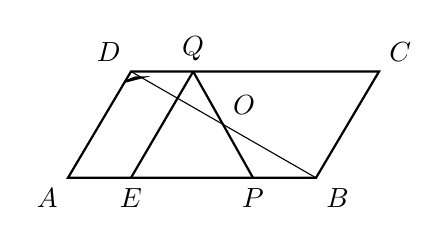
\begin{tikzpicture}[thick, scale=1]
  \coordinate (A) at (0.65,0);
  \coordinate (B) at (3.80,0);
  \coordinate (C) at (4.60,1.35);
  \coordinate (D) at (1.45,1.35);
  \coordinate (E) at (1.45,0);
  \coordinate (P) at (3.00,0);
  \coordinate (Q) at (2.24,1.35);
  \coordinate (O) at (2.617,0.677);

  \draw (A) -- (D) -- (C) -- (B) -- cycle;
  \draw (Q) -- (E);
  \draw (Q) -- (P);
  \draw[thin] (D) -- (B);

  \draw (1.373,1.221) -- (1.580,1.275) -- (1.504,1.274) -- (1.373,1.221);

  \node[below left] at (A) {$A$};
  \node[below right] at (B) {$B$};
  \node[above right] at (C) {$C$};
  \node[above left] at (D) {$D$};
  \node[below] at (E) {$E$};
  \node[below] at (P) {$P$};
  \node[above] at (Q) {$Q$};
  \node[above right] at (O) {$O$};
\end{tikzpicture}
\end{document}
